\documentclass[graybox]{svmult}

\usepackage{cite}
\usepackage[bottom]{footmisc}
\usepackage[utf8]{inputenc}
\usepackage{graphicx}
% epstopdf needs to be included after graphicx.
\usepackage{epstopdf}
\usepackage{listings}
\usepackage{makeidx}
\usepackage{multicol}
\usepackage{newtxtext}
\usepackage{newtxmath}
\usepackage{url}
\RequirePackage[l2tabu, orthodox]{nag}

% Allow PDF 1.7 documents to be included with \includegraphics
\pdfminorversion=7

\graphicspath{{./img/}}

% listing
\lstset{%
  language={C},
  basicstyle={\small\ttfamily},%
  identifierstyle={\small\ttfamily},%
  commentstyle={\small\itshape},%
  keywordstyle={\small\bfseries},%
  ndkeywordstyle={\small\ttfamily},%
  stringstyle={\small\ttfamily},%
  frame={tb},%
  breaklines=true,%
  columns=[l]{fullflexible},%
  numbers=left,%
  numberstyle={\scriptsize},%
  stepnumber=1,%
  numbersep=1em,%
  lineskip=-0.5ex,%
  mathescape,%
  xleftmargin=2em,%
  framexleftmargin=1.5em,%
}

\makeindex

\begin{document}

\title*{An MPI Framework for HPC Clusters Deployed with Software-Defined
Networking}
% Use \titlerunning{Short Title} for an abbreviated version of
% your contribution title if the original one is too long
\author{Keichi Takahashi, Susumu Date, Yasuhiro Watashiba, Yoshiyuki Kido,
Shinji Shimojo}
% Use \authorrunning{Short Title} for an abbreviated version of
% your contribution title if the original one is too long
\institute{Keichi Takahashi \at Nara Institute of Science and Technology,
8916-5 Takayama, Ikoma, Nara, Japan\\ \email{keichi@is.naist.jp}
\and Susumu Date, Yasuhiro Watashiba, Yoshiyuki Kido, Shinji Shimojo \at
Cybermedia Center, Osaka University, 5-1 Mihogaoka, Ibaraki, Osaka, Japan\\
\email{{date, watashiba-y, kido, shimojo}@cmc.osaka-u.ac.jp}}
\maketitle

\abstract*{Each chapter should be preceded by an abstract (no more than 200
words) that summarizes the content. The abstract will appear \textit{online}
at \url{www.SpringerLink.com} and be available with unrestricted access. This
allows unregistered users to read the abstract as a teaser for the complete
chapter. Please use the 'starred' version of the \texttt{abstract} command for
typesetting the text of the online abstracts (cf. source file of this chapter
template \texttt{abstract}) and include them with the source files of your
manuscript. Use the plain \texttt{abstract} command if the abstract is also to
appear in the printed version of the book.}

\abstract{Each chapter should be preceded by an abstract (no more than 200
words) that summarizes the content. The abstract will appear \textit{online}
at \url{www.SpringerLink.com} and be available with unrestricted access. This
allows unregistered users to read the abstract as a teaser for the complete
chapter.\newline\indent Please use the 'starred' version of the
\texttt{abstract} command for typesetting the text of the online abstracts
(cf. source file of this chapter template \texttt{abstract}) and include them
with the source files of your manuscript. Use the plain \texttt{abstract}
command if the abstract is also to appear in the printed version of the book.}

\section{Introduction}

The demand for computing performance of high-performance computing (HPC)
systems has been every-growing. In fact, exascale HPC systems are now on the
horizon. To meet the sustained growth of HPC systems, the high-performance
network that interconnects the computing nodes composing a cluster, or
\textit{interconnect}, needs to be enhanced to achieve larger scale, higher
bandwidth and lower latency. As a result, the interconnect now accounts for a
significant portion of total financial cost and power consumption of an HPC
system~\cite{Michelogiannakis2017}.

Until today, the established strategy to design a interconnect has been
\textit{over-provisioning}, where bandwidth and routes are over-provisioned to
accommodate any application with arbitrary communication pattern will not
experience degradation of communication performance. The reason for this
choice is two-fold: first, a production HPC system is usually shared by many
users, where each user runs different applications. Therefore, it is not
realistic to tailor an interconnect to a communication pattern of a single
application. Second, conventional networking hardware used in interconnects do
not allow administrators to change their configuration on-the-fly. Therefore,
the only choice is to over-provision the interconnect with abundant bandwidth
and routes. However, an over-subscribed design is becoming increasingly
challenging to implement due to its rapidly rising financial cost and power
consumption. We believe that dynamically controlling the traffic in the
interconnect based on the communication pattern of an application could
overcome this problem.

However, with the recent emergence of networking technologies that introduces
programmability into networks, the assumption that interconnects are static
and cannot be reconfigured does not hold anymore. A prominent example of such
networking technology is Software-Defined Networking (SDN), which is a novel
networking architecture that allows administrators to dynamically and flexibly
control the network like a software.

Based on this idea, we have been developing on \textit{SDN-enhanced MPI}, a
framework that integrates Software-Defined Networking (SDN) into Message
Passing Interface (MPI). The goal of this framework is to dynamically control
the traffic in the interconnect based on the MPI communication pattern of
applications by utilizing the network programmability provided by SDN\@. To
this end, we have demonstrated that individual MPI collectives are accelerated
by utilizing SDN~\cite{Dashdavaa2014,Takahashi2014}. In addition, we have
designed and implemented a mechanism to synchronize the progress of an
application and the reconfiguration of the
interconnect~\cite{Takahashi2015,Takahashi2018}. Furthermore, we have
developed a toolset consisting of (1) a profiler to extract communication
pattern from applications and (2) an interconnect simulator predict the
traffic flow generated in an interconnect~\cite{Takahashi2017}.

Although our work so far has demonstrated that individual MPI applications can
be accelerated through the application of SDN, a key issue has remained
towards the deployment on production clusters: our current SDN-enhanced MPI
framework does not allow the concurrent execution of multiple applications on
a cluster.

In this paper, we aim to solve this problem integrating our framework into the
job scheduler of a cluster.

The rest of this paper is organized as follows. Section~\ref{kt:sec:ii}
describes the key technologies behind the proposal and challenges to be tackled.
Section~\ref{kt:sec:iii} proposes the architecture of the proposed framework.
Section~\ref{kt:sec:iv} shows the preliminary evaluation result of the
proposed framework. Section~\ref{kt:sec:v} concludes this paper and discusses
future work.

\section{Background}\label{kt:sec:ii}

\subsection{Software-Defined Networking (SDN)}

Software-Defined Networking (SDN)~\cite{McKeown2008} is a novel networking
architecture that brings programmability into the network and allows users to
dynamically and flexibly control the network as if the network was a software.
In conventional networking architectures, the \textit{control plane}, which
makes the decision on how to handle packets, and the \textit {data plane},
which forwards packets, are tightly coupled together on each networking device
such as a switch. In SDN, the two planes are separated into different
hardware. Whereas data plane is implemented on each networking device, the
control plane is handled by a centralized software.

\subsection{Job Scheduler}

A job scheduler is a system that accepts \textit{job} submissions from users
and dispatch the

Examples of job schedulers used in production HPC systems include
Slurm~\cite{Yoo2003}, PBS
Professional\footnote{\url{https://www.pbspro.org/}},
Torque\footnote{\url{https://www.adaptivecomputing.com/products/torque/}} and
UNIVA Grid Engine\footnote{\url{http://www.univa.com/products/}}. In this
paper, Slurm is assumed as it is one of the most widely adopted open-source
job schedulers.

Figure~\ref{kt:fig:slurm} shows the architecture of Slurm. Slurm employs a
master-worker architecture like many other job schedulers. The master accepts
job requests from users and

Here, it is assumed
that the cluster has three types of node: login node, head node and compute
node.

Like many job
schedulers, Slurm employs a master-worker architecture, where the master
accepts from

\begin{figure}
    \centering
    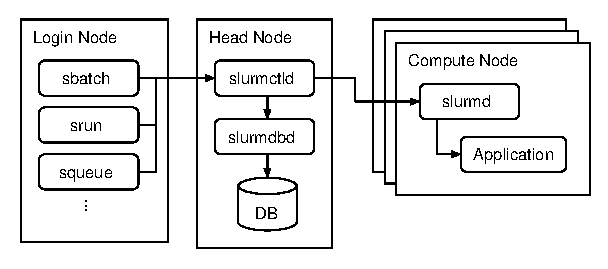
\includegraphics{slurm}
    \caption{Architecture of Slurm}%
    \label{kt:fig:slurm}
\end{figure}

\subsection{Challenges and Goal}

There are mainly two challenges in

\begin{itemize}
    \item Job start and finish:
    \item Node allocation and process mapping:
\end{itemize}


\section{Proposal}\label{kt:sec:iii}

\subsection{Overview}

Figure~\ref{kt:fig:architecture} shows the overall architecture of the
proposed SDN-enhanced MPI framework.

The scheduler plugin and the interconnect manager use
gRPC\footnote{\url{https://grpc.io/}} to communicate with one another. We have
chosen gRPC, which is an RPC framework built on top of HTTP/2, because it
can automatically generate server and client based on the interface
definition.

\begin{figure}
    \centering
    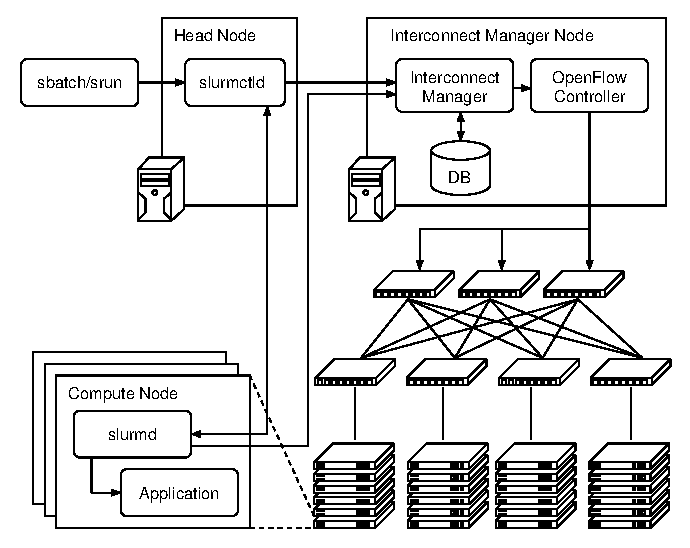
\includegraphics{architecture}
    \caption{Overall architecture}%
    \label{kt:fig:architecture}
\end{figure}

\subsection{Interconnect Manager}

The interconnect manager is responsible for computing and installing optimal
routes for each job.

\begin{itemize}
    \item Receiving notifications from srun and slurmd
    \item Persisting the state of jobs to a database
    \item Computing routes
    \item Installing routes to interconnect by talking to the OpenFlow
        controller.
\end{itemize}


The builtin REST API server of Ryu.

Ryu\footnote{\url{https://osrg.github.io/ryu/}}
SQLite\footnote{\url{https://www.sqlite.org/index.html}}

\subsection{Scheduler Plugin}

The scheduler plugin is responsible for

-

Slurm provides a plugin mechanism called Slurm Plug-in Architecture for Node
and job Control (SPANK). SPANK

Furthermore,

This plugin is inserted into srun and slurmd

srun: Sends job ID, name, uid/gid of user, number of tasks and communication
pattern name to the interconnect manager when a job is submitted.
slurmd: Sends job id, MPI rank, node ID and node name to interconnect manager
when a process consisting a job starts or exits. Blocks until the routings
have been setup in the interconnect.

\begin{lstlisting}
#!/bin/bash
#
#SBATCH --job-name=test_omp
#SBATCH --output=res_omp.txt
#
#SBATCH --ntasks=1
#SBATCH --cpus-per-task=4
#SBATCH --time=10:00
#SBATCH --mem-per-cpu=100
#SBATCH --comm-pattern=cg-c-128
\end{lstlisting}


\section{Preliminary Evaluation}\label{kt:sec:iv}

\subsection{Evaluation Environment}

\begin{figure}
    \centering
    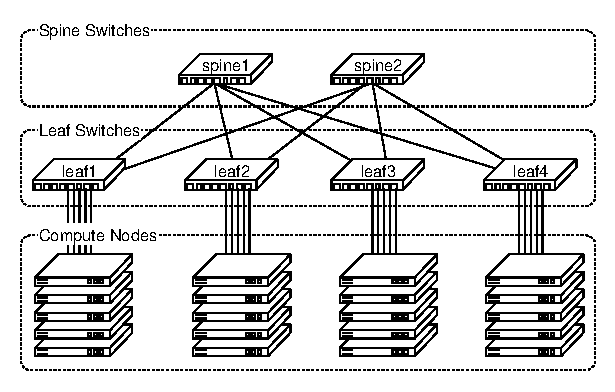
\includegraphics{evaluation_cluster}
    \caption{Cluster used for evaluation}%
    \label{kt:fig:cluster}
\end{figure}

\subsection{Evaluation Result}

\begin{figure}
    \centering
    \includegraphics{benchmark_result}
    \caption{Benchmark results using miniapps}%
    \label{kt:fig:benchmark}
\end{figure}

\section{Conclusion}\label{kt:sec:v}

\bibliographystyle{spmpsci}
\bibliography{references}

\end{document}
